%*******10********20********30********40********50********60********70********80

% For all chapters, use the newdefined chap{} instead of chapter{}
% This will make the text at the top-left of the page be the same as the chapter

\chap{Introduction}

In recent year there has been lot of research going on in area of deep learning. It has paved way for many abstruse problem in the field of computer vision. Convolution neural network have become so powerful that, they been able to object recognition better than human\cite{CNN-Better,krizhevsky2012imagenet,szegedy2015going,he2016deep,simonyan2014very}. Many researchers\cite{1608.08225} through empirical or statistical analysis have hypothesised why deep neural network work so very well.  had always  For many years deep learning used to be considered a black box as it has innumerable interacting, non linear parts. But recent progress was fueled by development of tools \cite{tensorflow2015-whitepaper} which enabled researchers to visualize and interpret the hidden layers of neural networks\cite{1506.06579}.
The CNN have shown excellent capability in classification task\cite{CNN-Better} but they require large amount of labeled data. Labeling and gathering large data require lot of human effort and money. This work tries to reduce this by developing generative model which are capable of generating labeled data.

\begin{figure}[H]
  \centering
    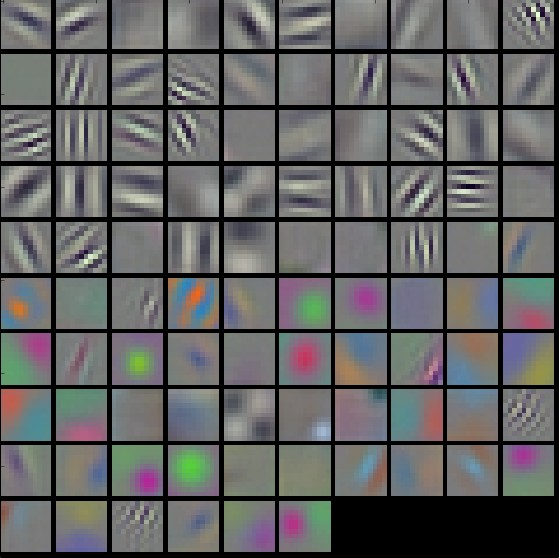
\includegraphics[scale=.3, angle=0]{Files/cnn_visaulize.jpeg}
    \caption[Typical-looking filters on the first CONV layer of a imagenet]{Typical-looking filters on the first CONV layer}
    \label{fig:visualize-cnn}
\end{figure}

\section{Synthetic Image Generation}
Image generation is one the key research area in field of computer vision. From statistical point of view we are trying to mimic distribution of a data-set. In this work we are trying to synthesis the images based on some given condition. Most widely used method before GAN used probabilistic generative models which are discussed in section 2.1.This work uses Generative Adversarial network framework for image generation .This technique was first introduced by ..... . been The paper proposed framework which was highly unstable and laked quality generated images.  This work focuses on the aspect of stabilising and reviewing the latest GAN frameworks.

